\documentclass{article}

%Package Part
\usepackage{relsize,setspace}  % used by latex(describe( ))
\usepackage{url}               % used in bibliography
\usepackage[superscript,nomove]{cite} % use if \cite is used and superscripts wanted
% Remove nomove if you want superscripts after punctuation in citations
\usepackage{lscape}            % for landscape mode tables
\textwidth 6.75in              % set dimensions before fancyhdr 
\textheight 9.25in
\topmargin -.875in
\oddsidemargin -.125in
\evensidemargin -.125in
\usepackage{fancyhdr}          % this and next line are for fancy headers/footers
\pagestyle{fancy}
\newcommand{\bc}{\begin{center}}  % abbreviate
\newcommand{\ec}{\end{center}}

\usepackage{Sweave}
\begin{document}

\Sconcordance{concordance:test.tex:test.Rnw:%
1 18 1 1 0 14 1 1 21 4 1 1 2 31 0 1 1 24 0 1 1 14 0 1 1 27 0 1 2 2 1 1 %
6 1 2 5 1 1 2 1 3 1 2 4 1 1 2 1 3 1 2 2 1 1 2 1 3 1 2 4 1 1 2 1 3 1 2 3 %
1 1 2 1 3 1 2 2 1 1 2 1 3 1 2 4 1 1 2 1 3 1 2 3 1 1 2 1 3 1 2 2 1 1 2 1 %
3 1 2 2 1}


%\SweaveOpts{width=6, height=4}


\title{Performance Analysis}
\author{}
\date{}

\setkeys{Gin}{width=1\textwidth}
\maketitle
%\tableofcontents


\section{Overview}
This documents go through performance of \verb|PS_12M_FWD|. Simulation period is from 2006-01-06 09:00:00 to 2013-01-11 09:00:00. The portfolio is composed with Large Caps (which hedge by Equity Trading Team in 'H' securities). Data source is WiseFN.

\subsection{Tables}
% latex table generated in R 2.15.2 by xtable 1.7-0 package
% Wed Jan 16 19:54:03 2013
\begin{table}[ht]
\begin{center}
\caption{Calendar Returns}
\begin{tabular}{rrrrrrrrr}
  \hline
 & 2006 & 2007 & 2008 & 2009 & 2010 & 2011 & 2012 & 2013 \\ 
  \hline
1 &  & -3.00 & -7.10 & 9.60 & -0.10 & -0.90 & 9.60 & -0.60 \\ 
  2 & 2.90 & 8.60 & 3.10 & -13.90 & 2.70 & -7.40 & 5.40 &  \\ 
  3 & 0.50 & 3.50 & 3.00 & 20.20 & 6.30 & -0.30 & -4.20 &  \\ 
  4 & 10.10 & 6.30 & 8.90 & 15.20 & 2.20 & 6.70 & -7.40 &  \\ 
  5 & -4.40 & 12.00 & 4.80 & 7.00 & -9.60 & -4.50 & -5.60 &  \\ 
  6 & -4.00 & 8.20 & -5.80 & -0.10 & 11.10 & 1.60 & 4.30 &  \\ 
  7 & -3.50 & 11.40 & -1.50 & 14.50 & 1.30 & 2.90 & 2.10 &  \\ 
  8 & 1.60 & 3.40 & -11.20 & 0.80 & -2.10 & -17.80 & 9.10 &  \\ 
  9 & 7.30 & 4.70 & 0.90 & 6.80 & 10.20 & -5.90 & 7.70 &  \\ 
  10 & 0.30 & 12.80 & -40.00 & -7.80 & 1.70 & 14.00 & -5.10 &  \\ 
  11 & 7.50 & -0.50 & 6.80 & -5.50 & 1.20 & -8.20 & 3.10 &  \\ 
  12 & 0.10 & 2.30 & 12.00 & 8.00 & 10.90 & 0.80 & 4.40 &  \\ 
  X1 & 18.70 & 94.20 & -32.90 & 62.10 & 39.60 & -20.50 & 23.40 & -0.60 \\ 
  X2 & 33.40 & 66.70 & -33.40 & 55.60 & 33.90 & -15.30 & -4.00 & 0.40 \\ 
  X3 & 5.80 & 47.60 & -50.60 & 36.90 & 23.00 & -17.00 & 0.40 & -0.60 \\ 
  X4 & 7.10 & 29.00 & -45.80 & 56.40 & 17.70 & -20.70 & 4.20 & 0.40 \\ 
  X5 & -2.00 & 30.90 & -38.40 & 26.00 & 27.50 & -1.70 & 1.30 & 0.30 \\ 
  best.bm & 12.50 & 48.20 & 14.90 & 8.60 & 14.10 & -8.80 & 10.90 & -0.10 \\ 
  best.worst & 4.10 & 24.10 & -2.20 & 11.60 & -7.30 & -31.20 & 4.00 & -1.50 \\ 
  KM1 & 5.70 & 32.20 & -38.30 & 51.80 & 22.70 & -13.30 & 11.40 & -0.50 \\ 
   \hline
\end{tabular}
\end{center}
\end{table}% latex table generated in R 2.15.2 by xtable 1.7-0 package
% Wed Jan 16 19:54:03 2013
\begin{table}[ht]
\begin{center}
\caption{Calendar Returns}
\begin{tabular}{rrrrrrrrr}
  \hline
 & 2006 & 2007 & 2008 & 2009 & 2010 & 2011 & 2012 & 2013 \\ 
  \hline
1 &  & -4.70 & -11.70 & 4.70 & -5.90 & 1.80 & 8.80 & -0.50 \\ 
  2 & -0.60 & 6.70 & 1.10 & -9.30 & -0.70 & -7.30 & 2.30 &  \\ 
  3 & 0.10 & -0.70 & 1.20 & 17.90 & 6.80 & 5.80 & 0.60 &  \\ 
  4 & 4.40 & 5.60 & 7.80 & 8.30 & 3.00 & 6.20 & -1.40 &  \\ 
  5 & -6.90 & 5.60 & 0.60 & 0.50 & -7.50 & -4.70 & -8.60 &  \\ 
  6 & -2.30 & 5.20 & -9.10 & 1.30 & 7.00 & -0.50 & 1.90 &  \\ 
  7 & 1.30 & 7.60 & -3.80 & 12.50 & 1.80 & 0.90 & -1.20 &  \\ 
  8 & 2.70 & 1.60 & -9.10 & 2.70 & -2.10 & -18.60 & 3.30 &  \\ 
  9 & 3.00 & 4.40 & 2.70 & 6.00 & 6.70 & 0.70 & 5.60 &  \\ 
  10 & 0.10 & 3.00 & -23.00 & -7.40 & 0.70 & 10.20 & -6.20 &  \\ 
  11 & 3.00 & -4.80 & -3.90 & -1.60 & 3.40 & -9.50 & 3.10 &  \\ 
  12 & 1.20 & -0.20 & 4.40 & 10.10 & 9.20 & 4.40 & 4.10 &  \\ 
  KM1 & 5.70 & 32.20 & -38.30 & 51.80 & 22.70 & -13.30 & 11.40 & -0.50 \\ 
   \hline
\end{tabular}
\end{center}
\end{table}% latex table generated in R 2.15.2 by xtable 1.7-0 package
% Wed Jan 16 19:54:04 2013
\begin{table}[ht]
\begin{center}
\caption{Annualized Returns}
\begin{tabular}{rrrrrrrrr}
  \hline
 & X1 & X2 & X3 & X4 & X5 & best.bm & best.worst & KM1 \\ 
  \hline
Annualized Return & 0.18 & 0.13 & -0.00 & 0.01 & 0.02 & 0.12 & -0.02 & 0.06 \\ 
  Annualized Std Dev & 0.31 & 0.30 & 0.25 & 0.26 & 0.24 & 0.15 & 0.20 & 0.25 \\ 
  Annualized Sharpe (Rf=0\%) & 0.56 & 0.43 & -0.01 & 0.05 & 0.08 & 0.84 & -0.09 & 0.22 \\ 
   \hline
\end{tabular}
\end{center}
\end{table}% latex table generated in R 2.15.2 by xtable 1.7-0 package
% Wed Jan 16 19:54:04 2013
\begin{table}[ht]
\begin{center}
\caption{Statistics}
\begin{tabular}{rrrrrrrrr}
  \hline
 & X1 & X2 & X3 & X4 & X5 & best.bm & best.worst & KM1 \\ 
  \hline
Observations & 366.00 & 366.00 & 366.00 & 366.00 & 366.00 & 366.00 & 366.00 & 366.00 \\ 
  NAs & 1.00 & 1.00 & 1.00 & 1.00 & 1.00 & 1.00 & 1.00 & 1.00 \\ 
  Minimum & -0.29 & -0.24 & -0.19 & -0.19 & -0.18 & -0.09 & -0.12 & -0.20 \\ 
  Quartile 1 & -0.02 & -0.02 & -0.02 & -0.02 & -0.01 & -0.01 & -0.02 & -0.02 \\ 
  Median & 0.01 & 0.01 & 0.00 & 0.00 & 0.00 & 0.00 & 0.00 & 0.00 \\ 
  Arithmetic Mean & 0.00 & 0.00 & 0.00 & 0.00 & 0.00 & 0.00 & 0.00 & 0.00 \\ 
  Geometric Mean & 0.00 & 0.00 & -0.00 & 0.00 & 0.00 & 0.00 & -0.00 & 0.00 \\ 
  Quartile 3 & 0.03 & 0.02 & 0.02 & 0.02 & 0.02 & 0.01 & 0.02 & 0.02 \\ 
  Maximum & 0.21 & 0.27 & 0.13 & 0.16 & 0.13 & 0.11 & 0.09 & 0.17 \\ 
  SE Mean & 0.00 & 0.00 & 0.00 & 0.00 & 0.00 & 0.00 & 0.00 & 0.00 \\ 
  LCL Mean (0.95) & -0.00 & -0.00 & -0.00 & -0.00 & -0.00 & 0.00 & -0.00 & -0.00 \\ 
  UCL Mean (0.95) & 0.01 & 0.01 & 0.00 & 0.00 & 0.00 & 0.00 & 0.00 & 0.01 \\ 
  Variance & 0.00 & 0.00 & 0.00 & 0.00 & 0.00 & 0.00 & 0.00 & 0.00 \\ 
  Stdev & 0.04 & 0.04 & 0.04 & 0.04 & 0.03 & 0.02 & 0.03 & 0.03 \\ 
  Skewness & -0.91 & -0.18 & -0.68 & -0.50 & -0.62 & 0.12 & -0.07 & -0.50 \\ 
  Kurtosis & 7.79 & 7.94 & 3.92 & 4.07 & 4.00 & 3.52 & 1.96 & 4.66 \\ 
   \hline
\end{tabular}
\end{center}
\end{table}
\subsection{Distribution}

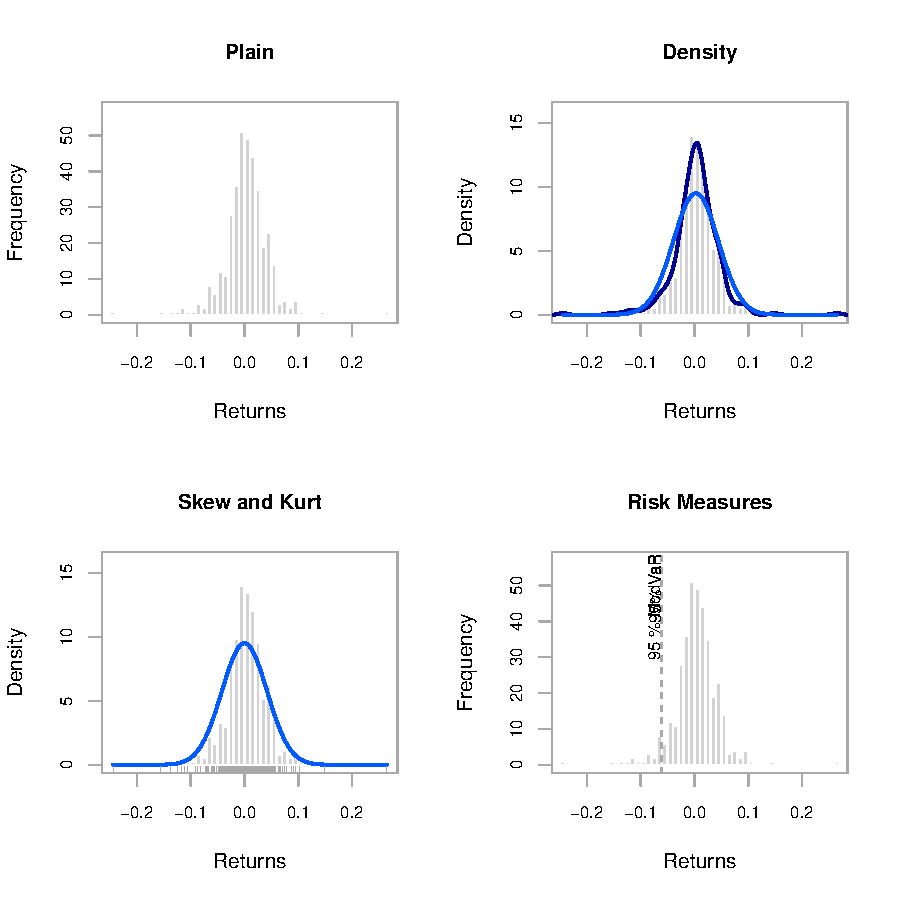
\includegraphics{graphics/plot-003}

\section{All yr Performance}
\setkeys{Gin}{width=0.5\textwidth}
%\begin{landscape}
\subsection{Returns}
\begin{tabular}{cc}
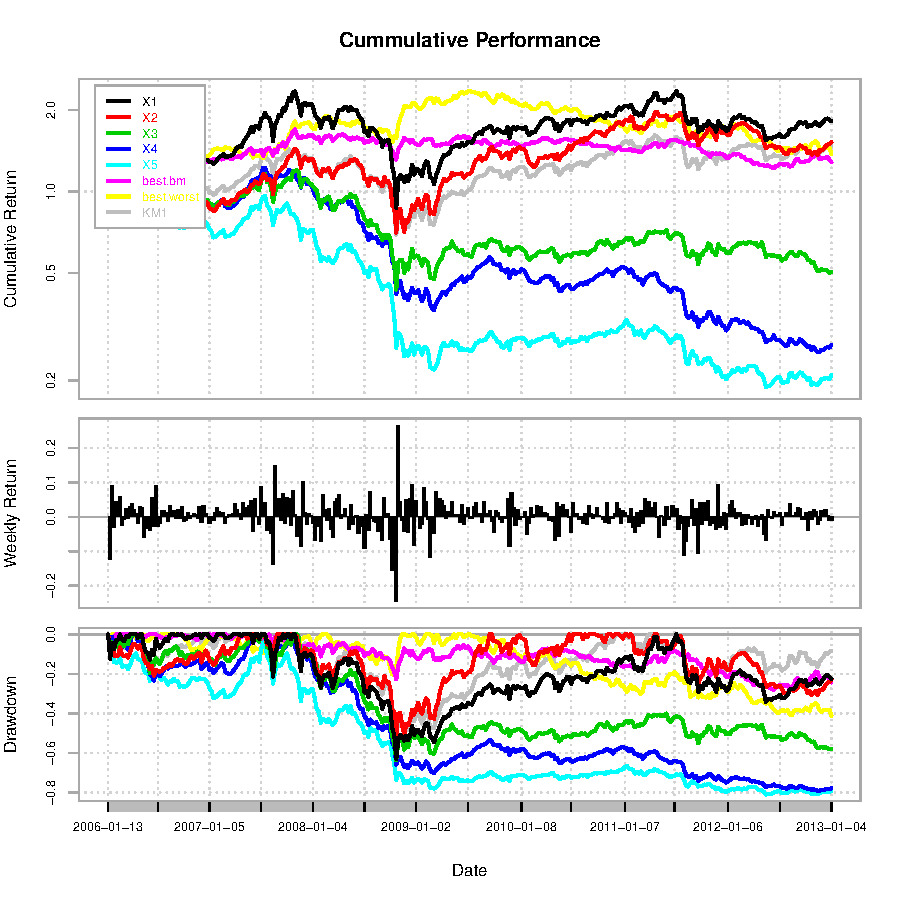
\includegraphics{graphics/plot-004}
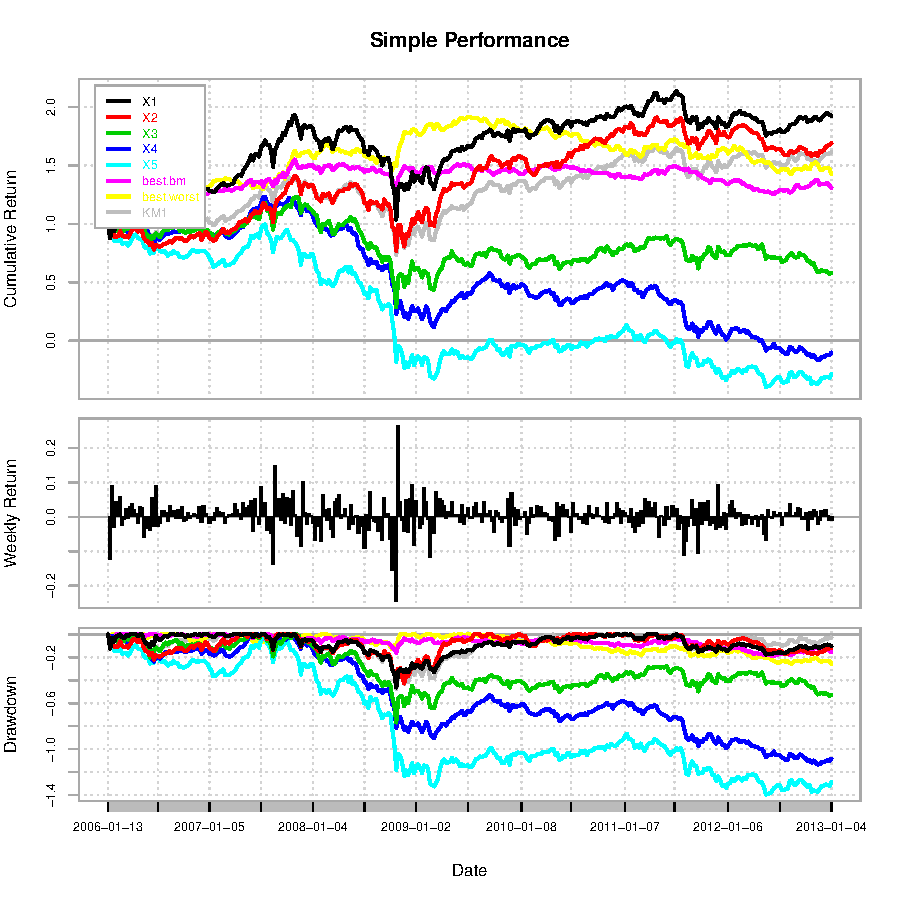
\includegraphics{graphics/plot-005}
\end{tabular}

%\end{landscape}
\subsection{Relative Returns}
\begin{tabular}{cc}
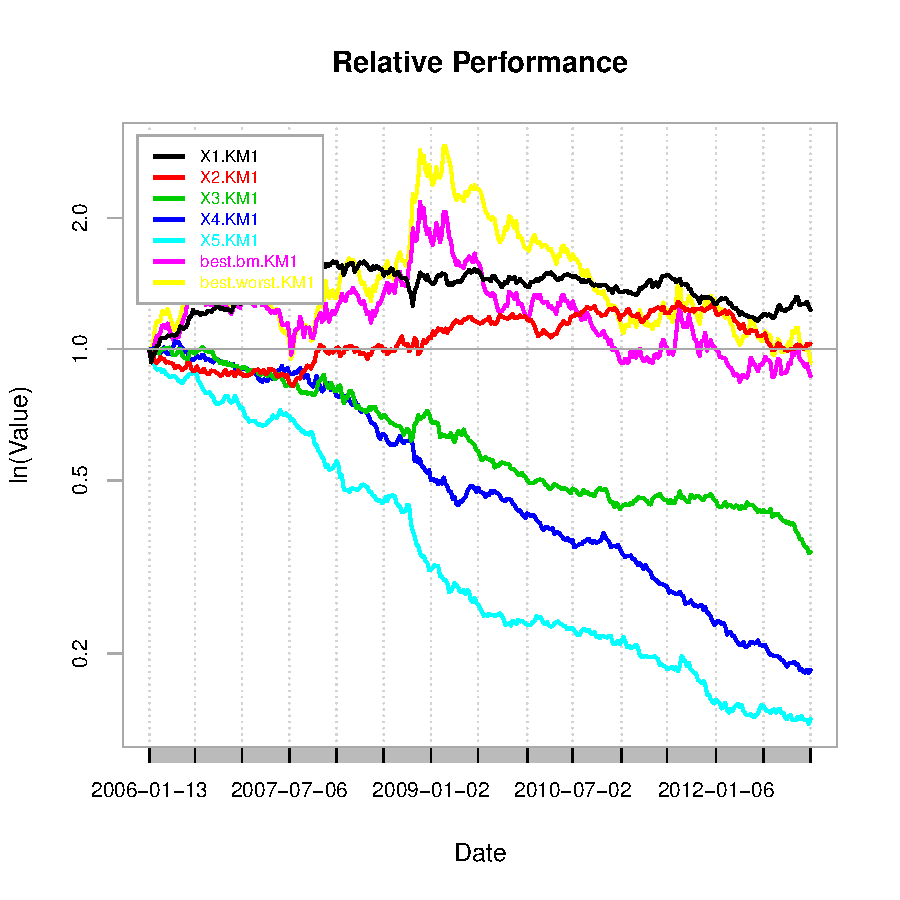
\includegraphics{graphics/plot-006}
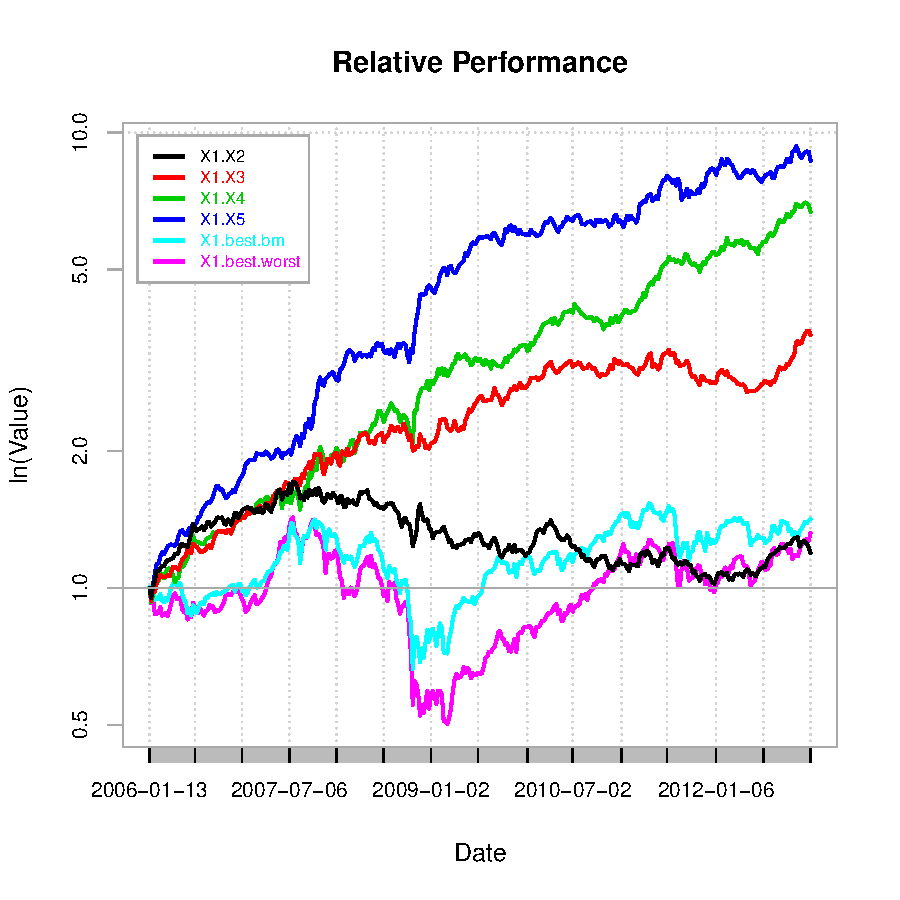
\includegraphics{graphics/plot-007}
\end{tabular}
\subsection{Other Charts}
\begin{tabular}{cc}
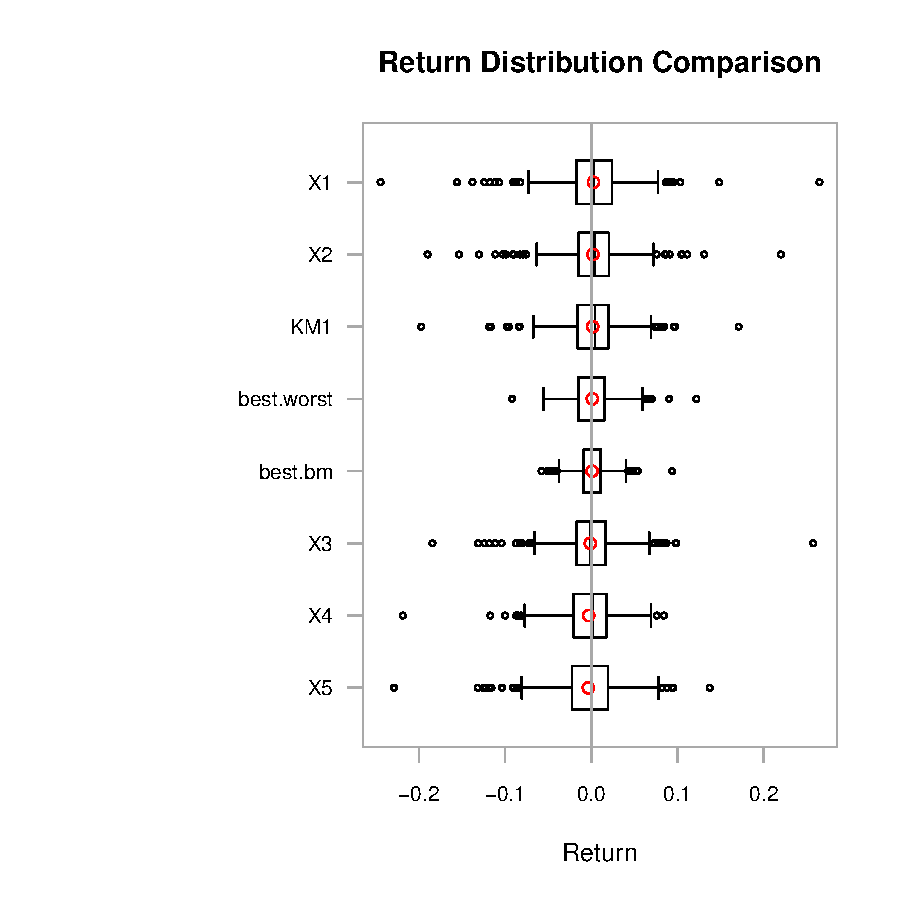
\includegraphics{graphics/plot-008}
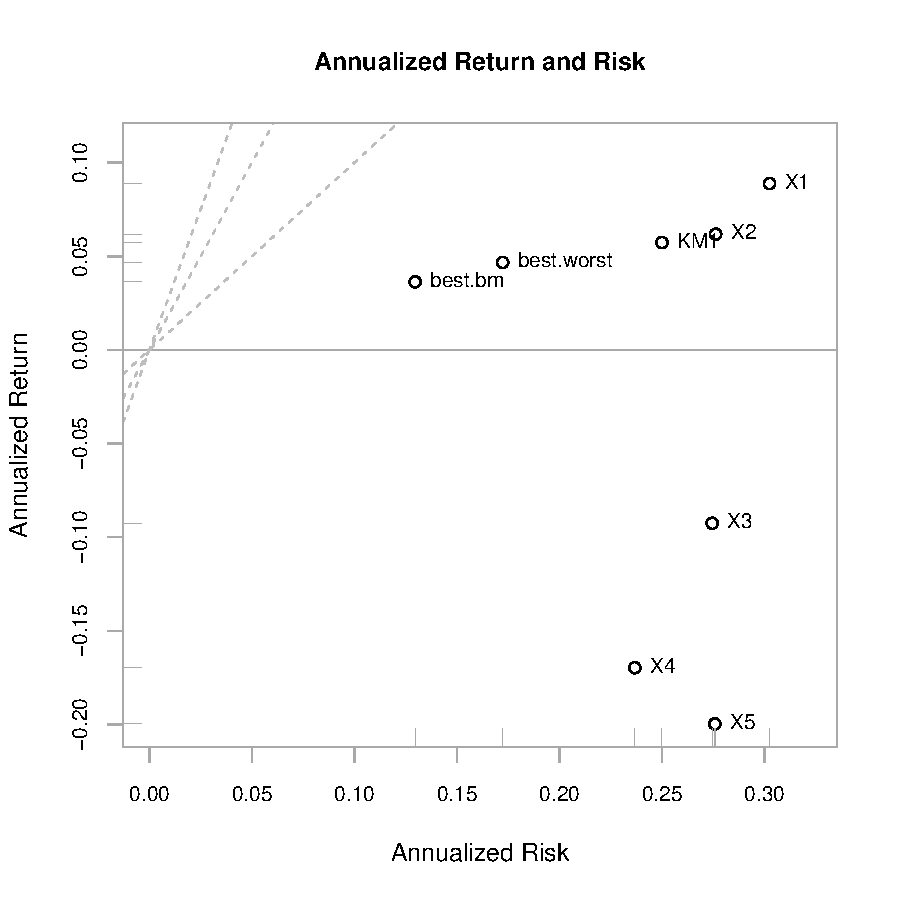
\includegraphics{graphics/plot-009}
\end{tabular}
\section{3yr Performance}
%\begin{landscape}
\subsection{Returns}
\begin{tabular}{cc}
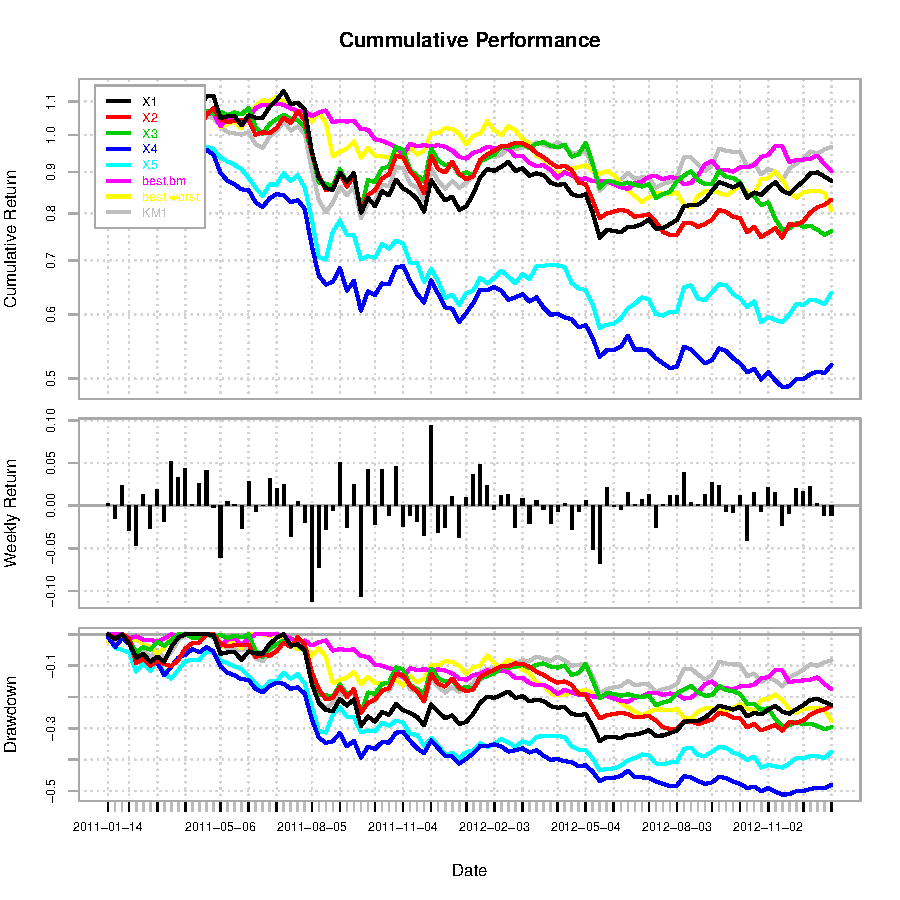
\includegraphics{graphics/plot-010}
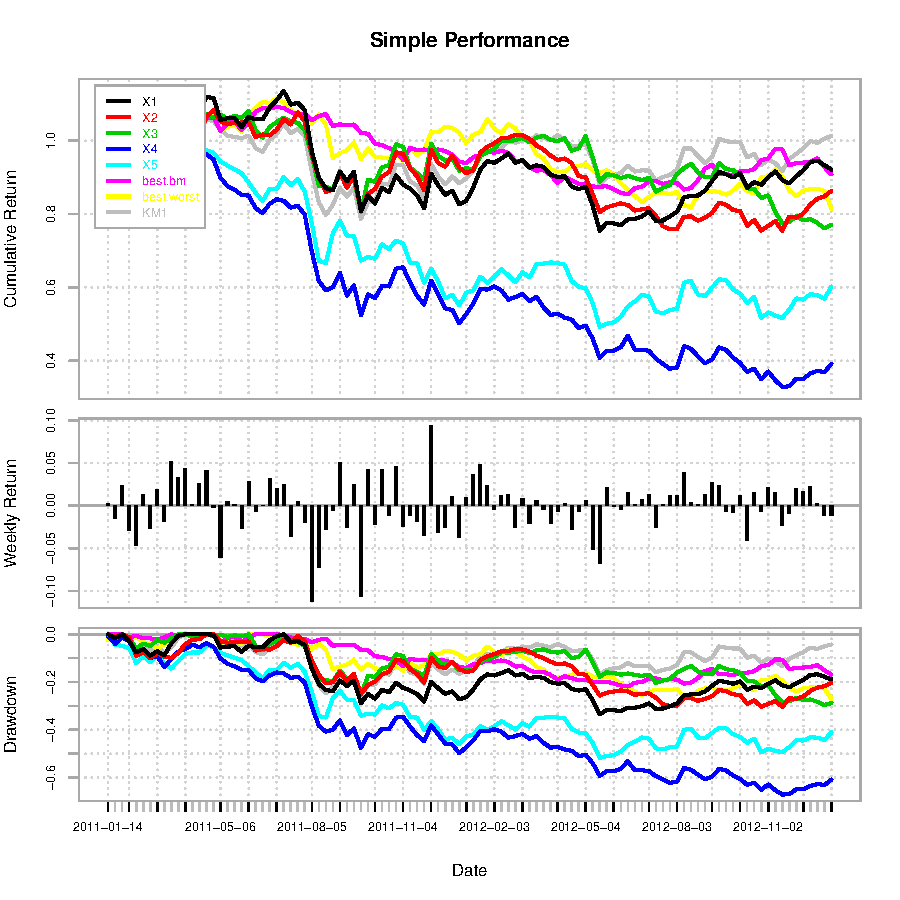
\includegraphics{graphics/plot-011}
\end{tabular}
%\end{landscape}
\subsection{Relative Returns}
\begin{tabular}{cc}
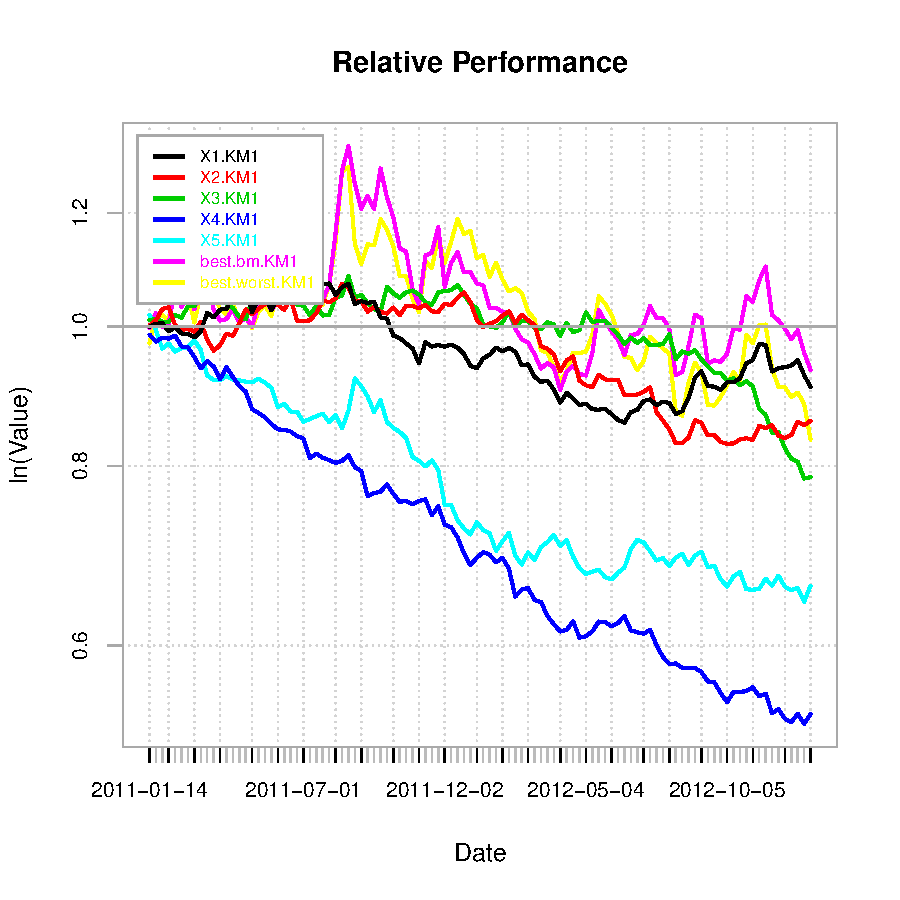
\includegraphics{graphics/plot-012}
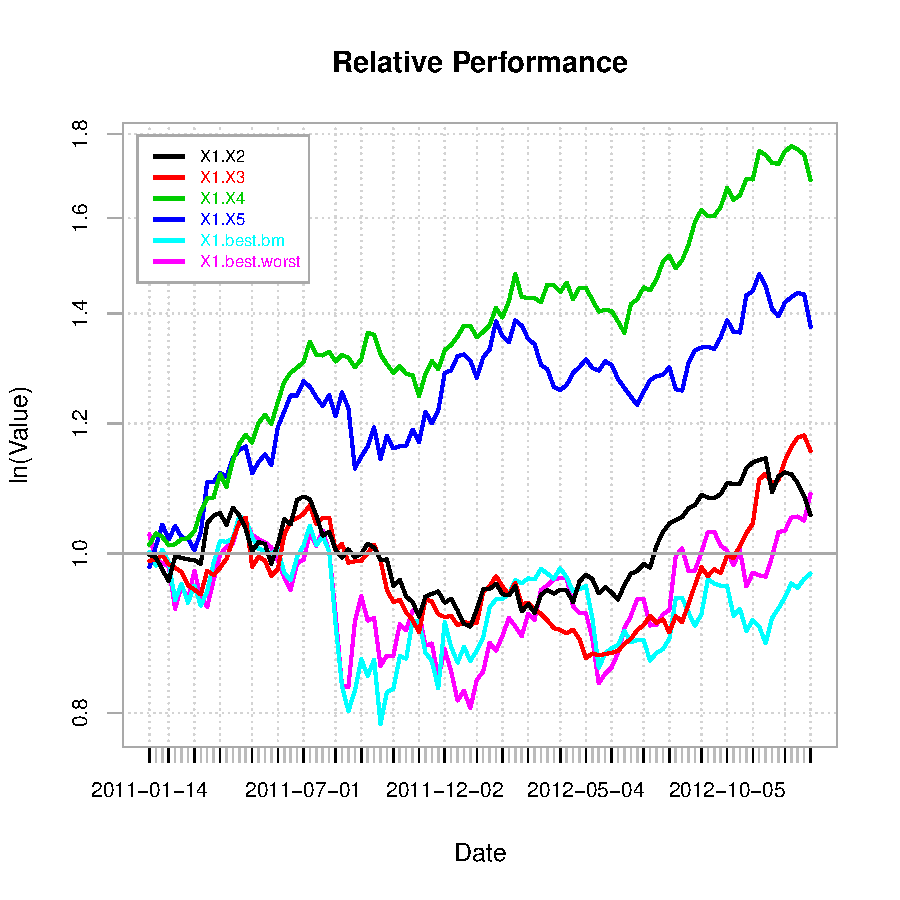
\includegraphics{graphics/plot-013}
\end{tabular}
\subsection{Other Charts}
\begin{tabular}{cc}
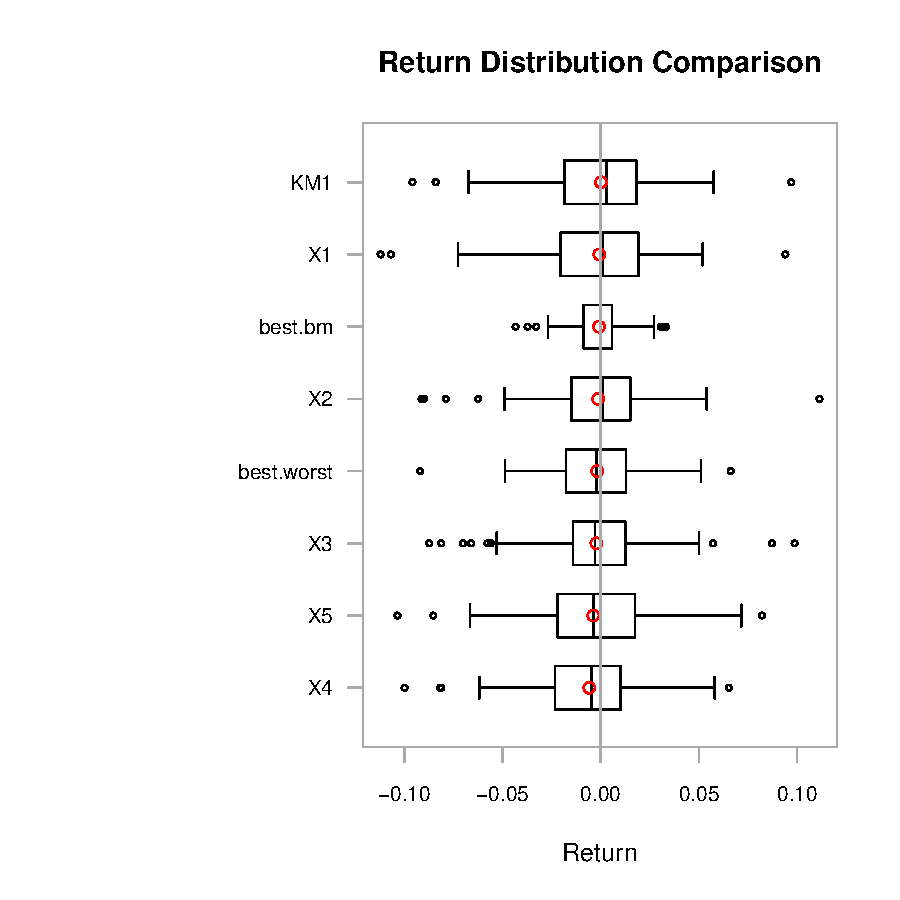
\includegraphics{graphics/plot-014}
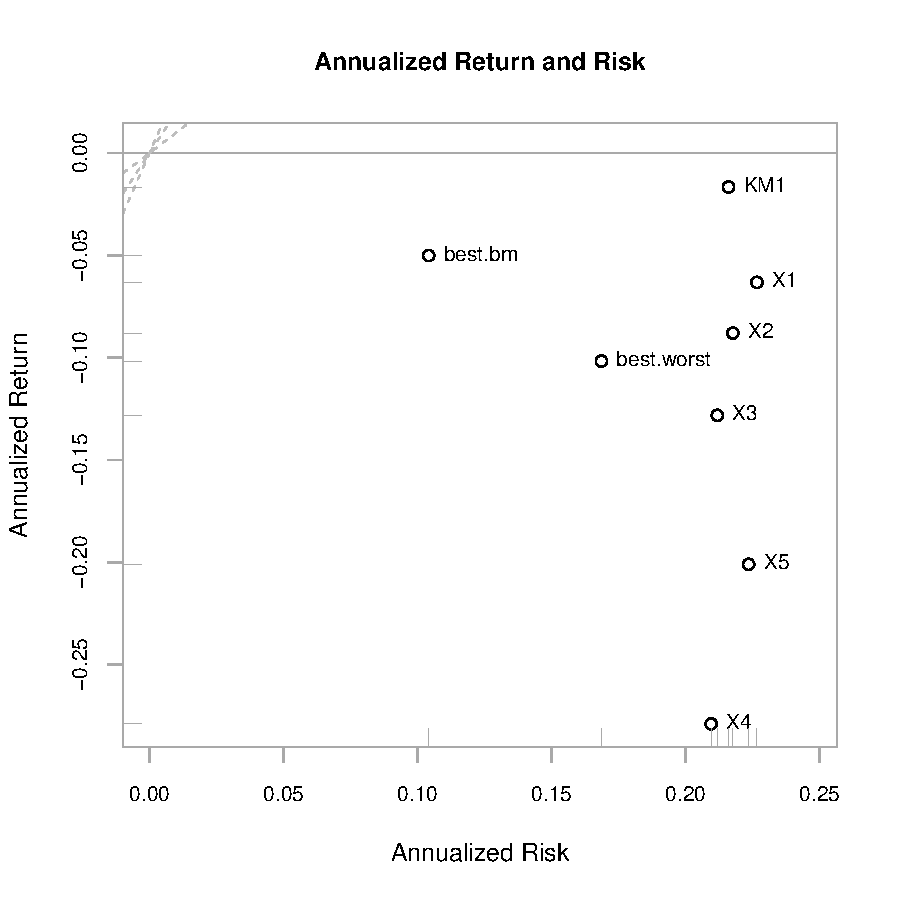
\includegraphics{graphics/plot-015}
\end{tabular}
\section{1yr Performance}
%\begin{landscape}
\subsection{Returns}
\begin{tabular}{cc}
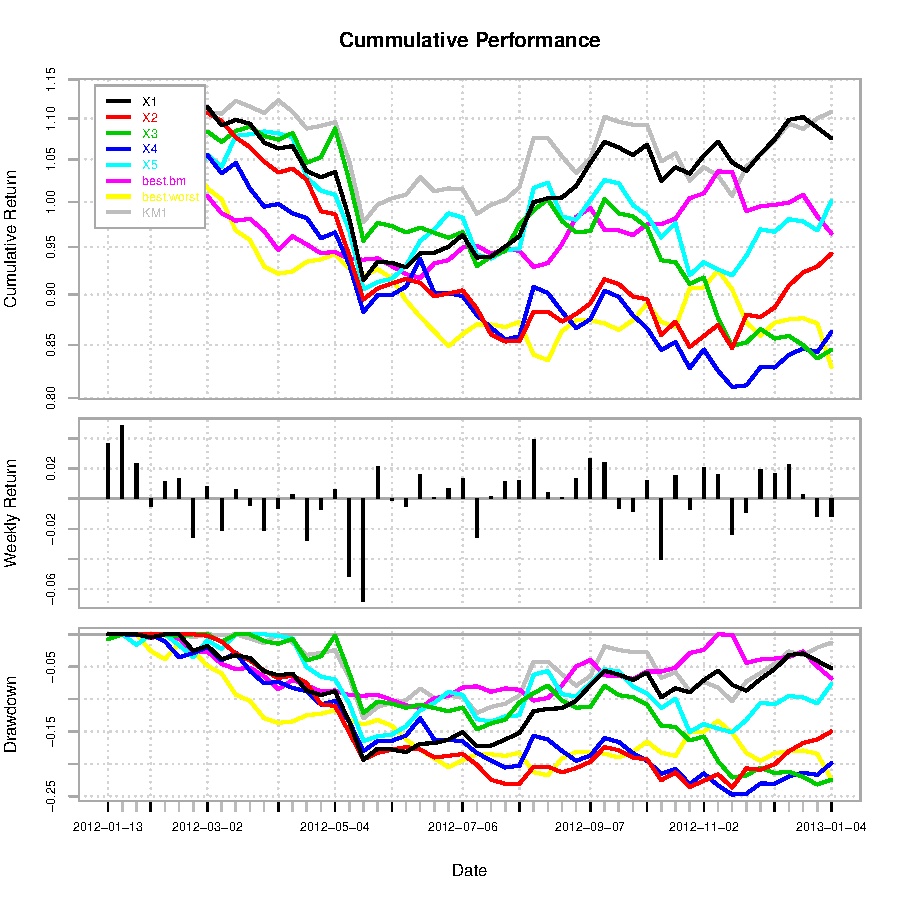
\includegraphics{graphics/plot-016}
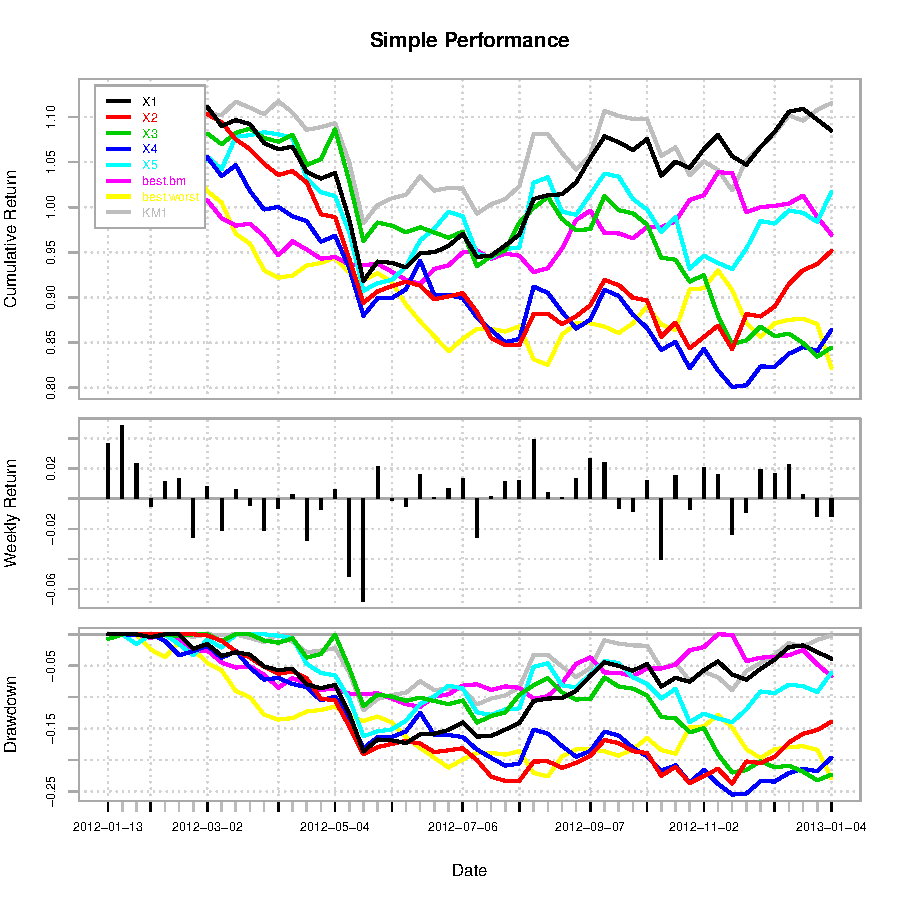
\includegraphics{graphics/plot-017}
\end{tabular}
%\end{landscape}
\subsection{Relative Returns}
\begin{tabular}{cc}
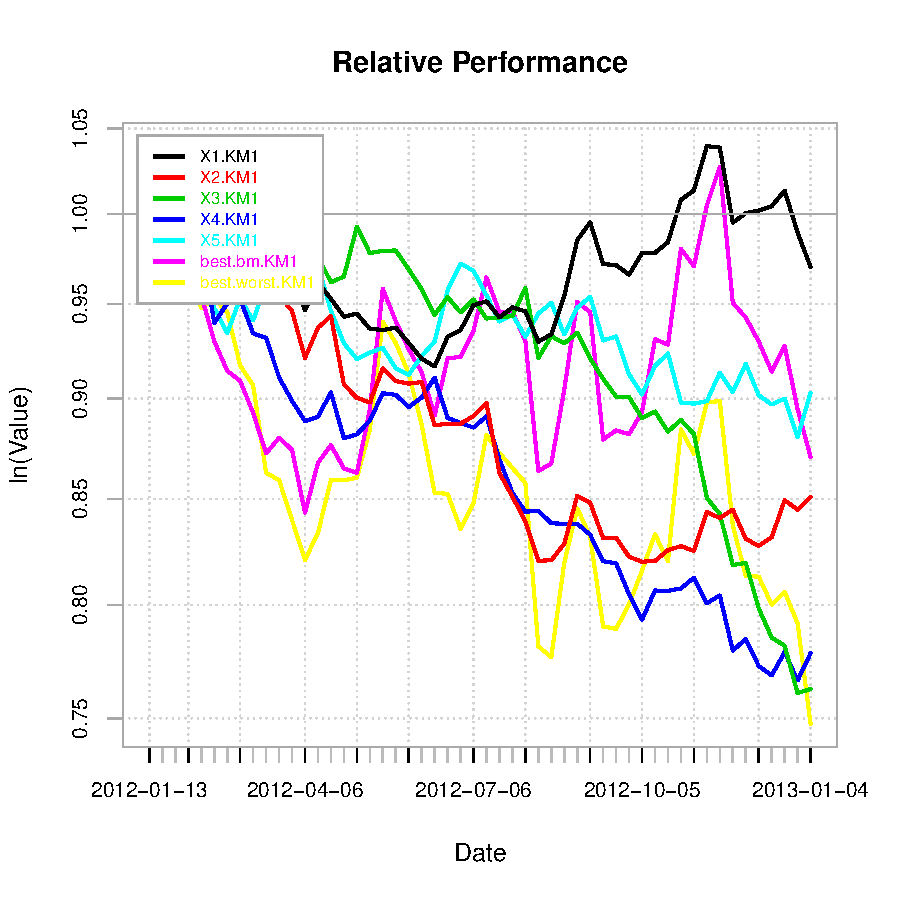
\includegraphics{graphics/plot-018}
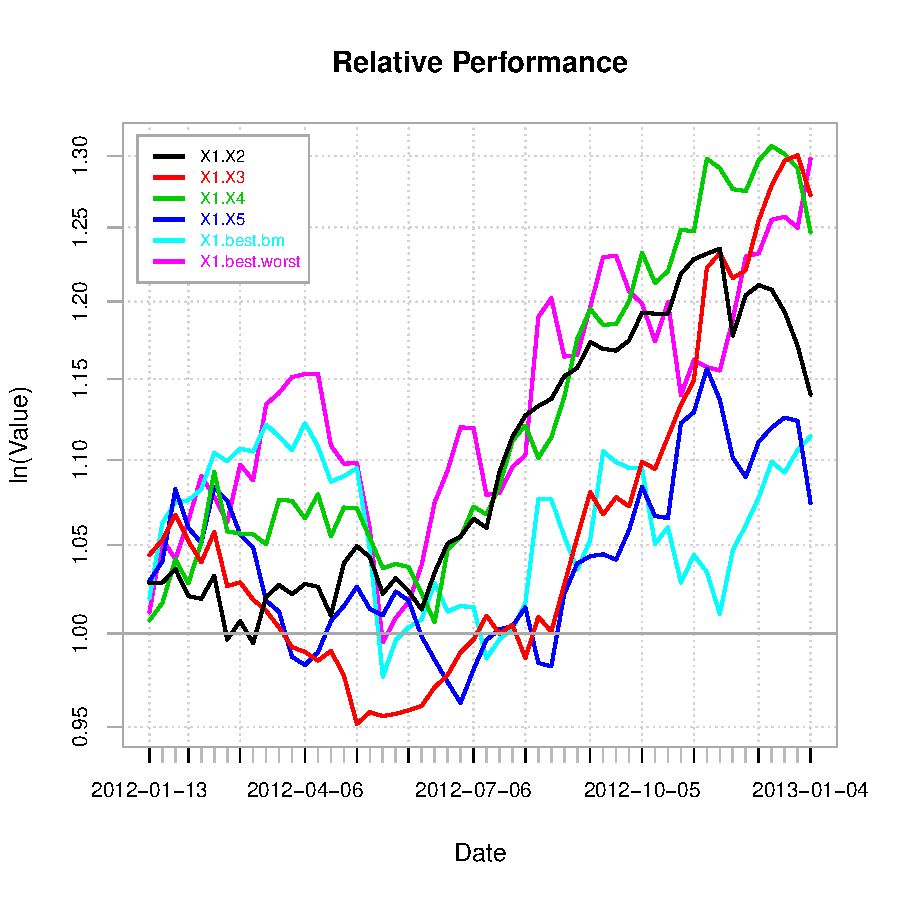
\includegraphics{graphics/plot-019}
\end{tabular}
\subsection{Other Charts}
\begin{tabular}{cc}
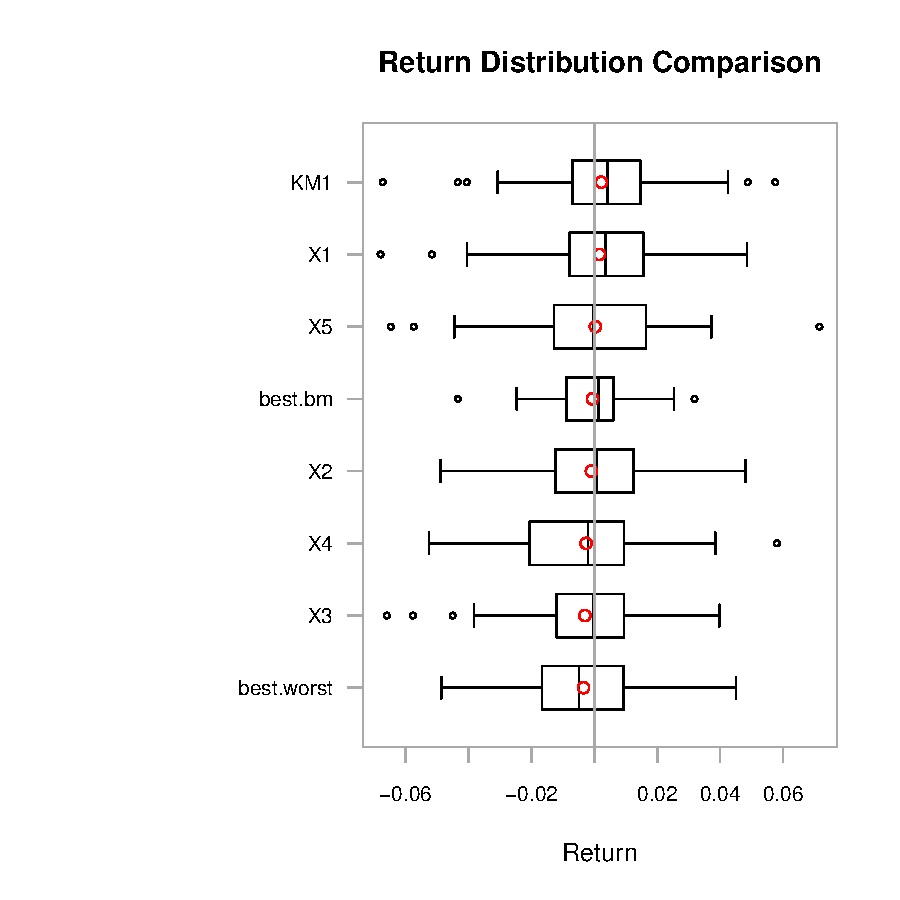
\includegraphics{graphics/plot-020}
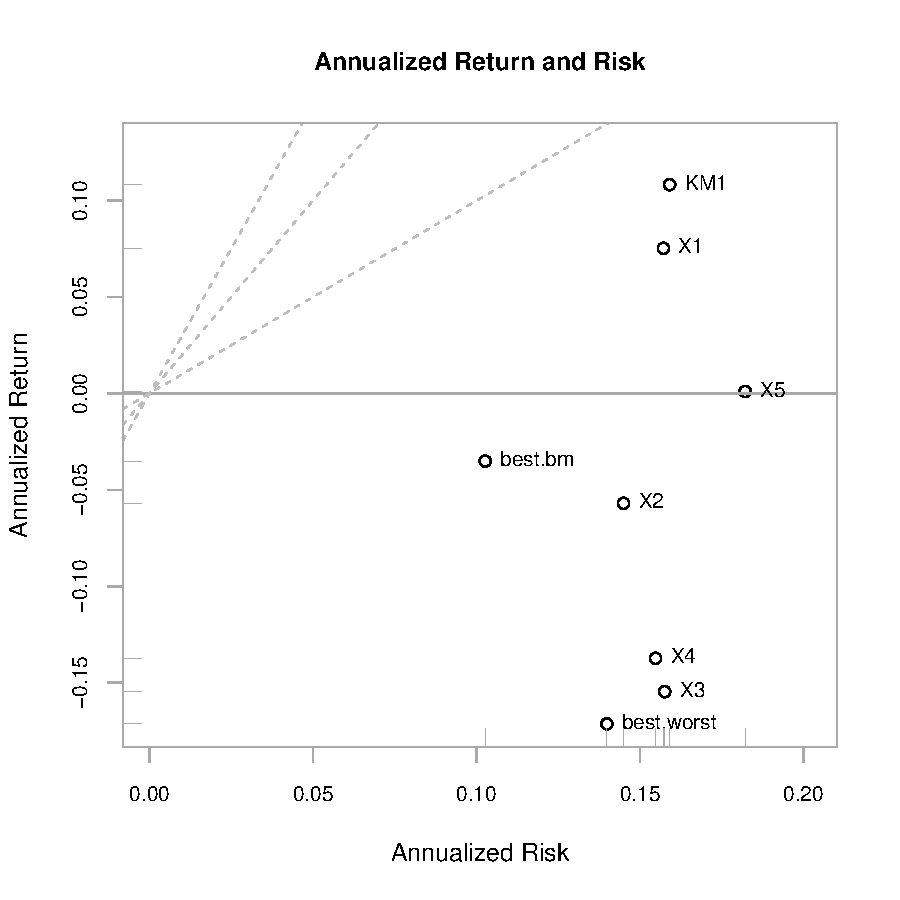
\includegraphics{graphics/plot-021}
\end{tabular}

\end{document}
